%!TEX root = ../report.tex

\section{Schnelligkeit}
Schnelligkeit ist die Fähigkeit in ermüdungsfreiem Zustand mit möglichst kurzen zeitlichem Abstand auf einen Reiz zu reagieren oder zu agieren.
\begin{figure}[H]
  \centering
  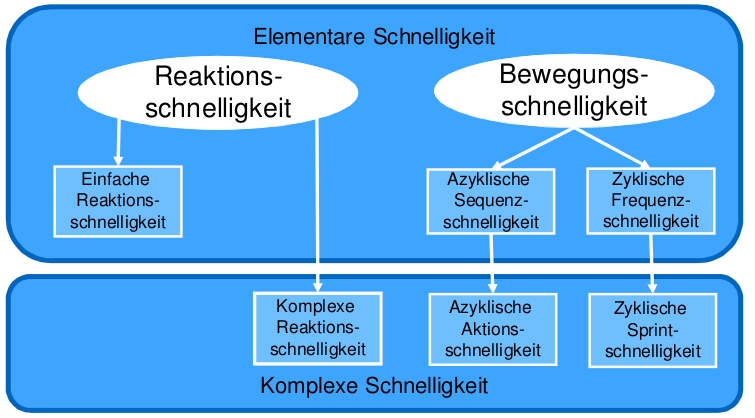
\includegraphics[width=.5\textwidth]{pictures/schnelligkeit_overview.png}
  \caption{Überblick Schnelligkeit}
\end{figure}
\begin{figure}[H]
  \centering
  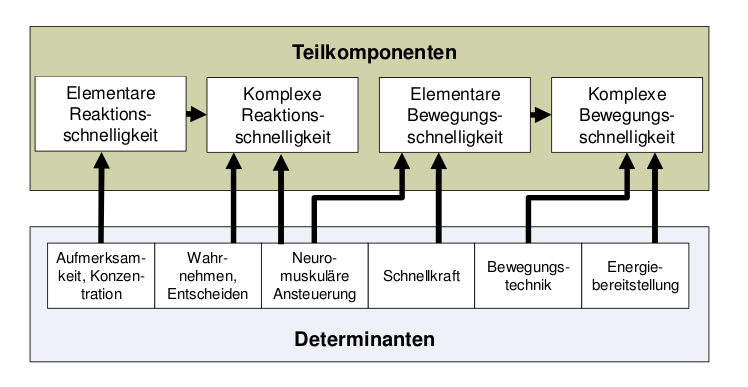
\includegraphics[width=.5\linewidth]{pictures/schnelligkeit_determinanten.png}
  \caption{Determinanten der Schnelligkeit}
\end{figure}

\subsection{Reaktionsschnelligkeit}
\begin{description}
  \item[Reaktionsfähigkeit] ist die psychophysische Fähigkeit auf Reize schnell zu reagieren.
  \item[Elementare Reaktionsschnelligkeit] Kleinmotorische Bewegungsantworten auf einfache Reize
  \item[Komplexe Reaktionsschnelligkeit] Großmotorische Bewegungsantworten \& komplexe (Wahl-) Reaktionen.
\end{description}

\subsubsection{Modell der Reaktionsgeschwindigkeit}
\begin{figure}[H]
  \centering
  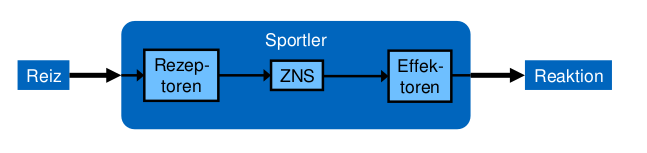
\includegraphics[width=.5\textwidth]{pictures/reaktionsgeschwindigkeit_modell.png}
  \caption{Modell der Reaktionsgeschwindigkeit}
\end{figure}
\begin{description}
    \item[Übertragung bis Rezeptor] hängt vorwiegend von den Eigenschaften des Rezeptors ab (1-20ms).
    \item[Restliche ÜBertragung] wird von den Eigenschaften des Nervensystems beeinflusst (Rezeptor $\rightarrow$ ZNS: 1-100ms, ZNS $\rightarrow$ Effektor: 10-20ms).
    \item[Verarbeitung im ZNS] wird beeinflusst von psychischen Eigenschaften wie Aufmerksamkeit und Wahrnehmung und kann von 70 bis 300ms dauern.
    \item[Verarbeitung in den Effektoren] Abhängig von neuromuskulären Eigenschaften wie Fastetypzusammensetzung oder inter-/intramuskuläre Koordination
\end{description}
Die gesammte Übertragungszeit beträgt in etwa 112 - 510ms.

\subsection{Bewegungsschnelligkeit}
Bewegungsschnelligkeit ist die Fähigkeit, Bewegungen in höchster Geschwindigkeit oder kürzester Zeit auszuführen.
\begin{figure}[H]
    \centering
    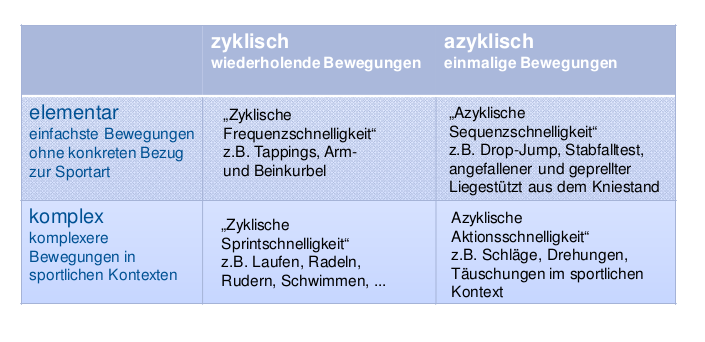
\includegraphics[width=.7\textwidth]{pictures/bewegungsgeschwindigkeit_struktur.png}
    \caption{Struktur der Bewegungsschnelligkeit}
\end{figure}

Die Bewegungsschnelligkeit hängt von drei Bereichen ab:
\begin{description}
    \item[Neuromuskuläres System] Neuronale Steuer- \& Regelprozesse, Reaktionsgeschwindigkeit, inter/intra-muskuläre Koordination,\ldots
    \item[Psychisches System] Konzentration, Wahrnehmung, Motivation, \ldots
    \item[Tendomuskuläres System] Querschnittsfläche FT-Fasern, Stiffness, Viskosität, \ldots
\end{description}
